
Случайный вектор ($\xi$, $\eta$) имеет равномерное распределение в области $D$:
\[
    D=\begin{pmatrix}4x-2y\geqslant2,\\x\leqslant3,y\geqslant1\end{pmatrix}
\]
$\zeta=2\xi^4-2$, $\nu=\lfloor5\eta\rfloor$, $\mu= -8\xi+4\eta$.

\begin{sympycode}
x, y, z = symbols('x y z')
xi, eta = symbols('xi eta')
x2 = 3
y1 = 1
line_eq = 4*x - 2*y - 2
yto = solve(line_eq, y)[0]
xfrom = solve(line_eq, x)[0]
x1 = xfrom.subs(y, y1)
y2 = yto.subs(x, x2)
D = And(line_eq >= 0, x <= x2, y >= y1)
x_interval = Interval(x1, x2)
y_interval = Interval(y1, y2)
x_interval_by_y = Interval(xfrom, x2)
y_interval_by_x = Interval(y1, yto)
zeta = 2 * xi ** 4 - 2
nu = floor(5 * eta)
mu = -8 * xi + 4 * eta
\end{sympycode}

\begin{figure}[h!]
    \centering
    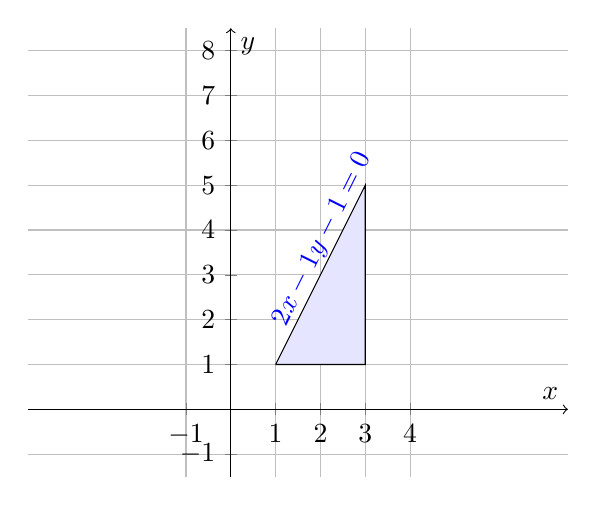
\begin{tikzpicture}
        \begin{axis}[
                xlabel=$x$,
                ylabel=$y$,
                xmin=-1.5, xmax=4.5,
                ymin=-1.5, ymax=8.5,
                axis lines=middle,
                axis line style={->},
                % ticks=none,
                clip=true,
                xtick={-1,0,1,2,3,4},
                ytick={-1,0,1,2,3,4,5,6,7,8},
                axis equal,
                grid=both,
            ]
            \addplot[fill=blue!10] coordinates {(1,1) (3, 5) (3, 1) (1,1)};
            % \addplot[domain=1:3, blue, dashed] {2*x-1};
            \node[blue, right, rotate=63.435] at (axis cs: 1, 1.7) {$2x-1y-1=0$};
        \end{axis}
    \end{tikzpicture}
    \caption{Область $D$}
    \label{fig:D}
\end{figure}

